% magarray: how the board's host side behaves. Build: latexmk -lualatex magarray.tex
\documentclass[aspectratio=169,11pt]{beamer}
\usetheme[progressbar=frametitle]{moloch}
\usepackage{fontspec}
\setsansfont{FiraSans}[Extension=.otf, UprightFont=*-Light, BoldFont=*-Regular, ItalicFont=*-LightItalic, BoldItalicFont=*-Italic]
\setmonofont{FiraMono}[Extension=.otf, UprightFont=*-Regular, BoldFont=*-Medium, Scale=0.85]
\usefonttheme{professionalfonts}
\usepackage{booktabs, array}
\newcolumntype{P}[1]{>{\raggedright\arraybackslash}p{#1}}
\usepackage[per-mode=symbol, mode=text]{siunitx}
\usepackage{tikz}
\usetikzlibrary{arrows.meta, positioning}
\usepackage{listings}
\definecolor{ink}{HTML}{0B0B0B}\definecolor{ink2}{HTML}{52514E}\definecolor{rule}{HTML}{D9D8D3}
\definecolor{surface}{HTML}{FCFCFB}\definecolor{panel}{HTML}{F0EFEC}\definecolor{accent}{HTML}{2A78D6}
\setbeamercolor{normal text}{fg=ink, bg=surface}\setbeamercolor{frametitle}{fg=surface, bg=ink}
\setbeamercolor{progress bar}{fg=accent, bg=rule}\setbeamercolor{block title}{fg=ink, bg=panel}\setbeamercolor{block body}{fg=ink, bg=panel!45}
\lstset{basicstyle=\ttfamily\scriptsize, columns=fullflexible, keepspaces=true, breaklines=true}
\tikzset{stage/.style={draw=rule, fill=panel, rounded corners=2pt, font=\scriptsize\ttfamily, minimum height=6mm, inner xsep=4pt},
         flow/.style={-{Stealth[length=4pt]}, draw=ink2, line width=0.6pt}}

\title{magarray}
\subtitle{The host side of the 5×5 LIS3MDL board: what it sends, how it is read, recorded and replayed}
\author{Arshia}
\date{15 November 2026}

\begin{document}
\maketitle

\begin{frame}{What it is, and what it is not}
  \begin{columns}[T]
    \begin{column}{0.5\textwidth}
      \begin{block}{In}
        the wire protocol, measured on the bench; a decoder; a recorder that keeps every read with its arrival time; replay; a Qt grid for bring-up. Python and C++, tested on the same captures.
      \end{block}
    \end{column}
    \begin{column}{0.46\textwidth}
      \begin{block}{Out}
        calibration, geometry, the robot, navigation: those are \texttt{mipe}'s. No dependency on it.
      \end{block}
      \begin{block}{Receive only}
        nothing writes to the board; DTR and RTS held low; the port locked, so a second reader waits instead of splitting bytes.
      \end{block}
    \end{column}
  \end{columns}
\end{frame}

\begin{frame}{The wire, on one slide}
  \footnotesize
  \texttt{FA 70 | type | id | len u16 | payload | sum u16} \quad (behind the center board, wrapped in \texttt{AD 69 | AA | channel | len | board frame | sum})
  \vspace{2mm}
  \begin{tabular}{@{}lP{8.8cm}l@{}}
    \toprule
    & & evidence \\
    \midrule
    scan (type 0x54) & u32 ticks, then per sensor: id, x, y, z, w as i16; 25 sensors, 237 bytes & bench \\
    rate & \SI{80.1}{\hertz}; ticks +12 per scan, never missing; \SI{960}{ticks/s}, \SI{+1.6}{ppm} against the host & bench \\
    per sensor & about \SI{40}{\hertz} on its own oscillator: half the readings repeat; a reading is up to \SI{25}{\milli\second} old & bench \\
    counts & $\pm$\SI{4}{gauss}, 6842 counts/gauss, \SI{14.6}{\nano\tesla} a count; saturation at 32767 & fit, twice \\
    latency & a fresh reading describes the field about \SI{37}{\milli\second} before it arrives & fit, two sessions \\
    axes & right-handed; $x = -x$, $y = +y$, $z = -z$ of the board's grid, each sensor within 1–3° & fit, Earth's field \\
    unknown & how a scan's 25 reads spread in time; the firmware's registers; what $w$ is for & \\
    \bottomrule
  \end{tabular}
  \vspace{2mm}

  Receiving: find the sync; bound \texttt{len}; check the sum; after a failure resync one byte later; validate the structure; count everything. A lost link looks like junk, not silence.
\end{frame}

\begin{frame}{The shape: the same as every device mipe drains}
  \begin{center}
  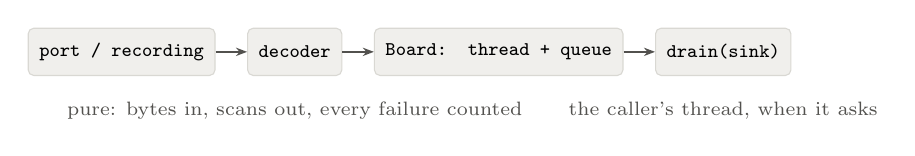
\begin{tikzpicture}[node distance=4mm]
    \node[stage] (src) {port / recording};
    \node[stage, right=of src] (dec) {decoder};
    \node[stage, right=of dec] (board) {Board: thread + queue};
    \node[stage, right=of board] (drain) {drain(sink)};
    \draw[flow] (src) -- (dec); \draw[flow] (dec) -- (board); \draw[flow] (board) -- (drain);
    \node[font=\scriptsize, text=ink2, below=2mm of dec] {pure: bytes in, scans out, every failure counted};
    \node[font=\scriptsize, text=ink2, below=2mm of drain] {the caller's thread, when it asks};
  \end{tikzpicture}
  \end{center}
  \begin{columns}[T]
    \begin{column}{0.5\textwidth}
      \begin{block}{Inside: push}
        the reader thread reads with a timeout, stamps the arrival (steady clock, ns), tees the bytes to the recording, decodes, queues; the queue is bounded and counts what it drops; it reconnects by itself.
      \end{block}
    \end{column}
    \begin{column}{0.46\textwidth}
      \begin{block}{Outside: pull}
        \texttt{wait\_for}, then \texttt{drain(sink)}: every queued scan, oldest first. \texttt{replay(path, sink)} is the same decoder on a recording, each scan stamped with its recorded arrival. Live and replay are one code path.
      \end{block}
    \end{column}
  \end{columns}
\end{frame}

\begin{frame}[fragile]{The recording: every read, with its arrival}
  \begin{columns}[T]
    \begin{column}{0.5\textwidth}
      \footnotesize
      \texttt{.bsr}: \\
      magic \texttt{BSTREAM1} · int64 steady ns at start · int64 system ns at start · u32 + JSON note \\
      then records: int64 arrival ns · u32 length · bytes
      \vspace{2mm}
      \begin{itemize}
        \item unbuffered: a kill loses nothing written
        \item never replaced without \texttt{--overwrite}; empty files removed
        \item legacy \texttt{.chunks} and \texttt{.bin} still read; nothing writes them
        \item the capsule's recorder is to write the same format
      \end{itemize}
    \end{column}
    \begin{column}{0.46\textwidth}
      \begin{block}{Why reads, not just bytes}
        a recording replays through the decoder exactly as the live stream did, and the arrival times let the board's clock be mapped onto the host's afterwards (the lower envelope of arrival against ticks). The two clocks in the header make it comparable with the arm's \texttt{.ecraw}.
      \end{block}
    \end{column}
  \end{columns}
\end{frame}

\begin{frame}[fragile]{Using it}
  \begin{columns}[T]
    \begin{column}{0.48\textwidth}
      \textbf{Python}
\begin{lstlisting}
magarray record raw/board0 --port /dev/serial/by-id/usb-Silicon_Labs_CP2102...
magarray info raw/board0.bsr
magarray view --file raw/board0.bsr --loop

from magarray.recording import read
from magarray.wire import StreamDecoder
rec = read("raw/board0.bsr"); d = StreamDecoder()
for t_ns, data in rec.records:
    scans = d.feed(data, t_ns / 1e9)
\end{lstlisting}
    \end{column}
    \begin{column}{0.48\textwidth}
      \textbf{C++}
\begin{lstlisting}
add_subdirectory(external/magarray/cpp)
target_link_libraries(app PRIVATE magarray::magarray)

magarray::BoardOptions o;
o.open = [] { return magarray::open_serial("/dev/ttyUSB1"); };
o.record = "raw/board0";
magarray::Board board(o);
board.wait_for(100ms);
board.drain([](const magarray::Scan& s) { ... });
magarray::replay("raw/board0.bsr", sink);
\end{lstlisting}
    \end{column}
  \end{columns}
  \vspace{1mm}
  \footnotesize Tested: 27 Python and 19 C++ tests on the same captures; the two decoders agree scan for scan. Linux only; the serial port is the one platform piece.
\end{frame}

\end{document}
